
\documentclass{article}
\usepackage[utf8]{inputenc}
\usepackage{graphicx}
\usepackage{subcaption}
\usepackage{tikz} 
 \usetikzlibrary{arrows,automata,positioning,petri}
 
\title{Report on Labwork 7}
\author{TRAN Thi Hong Hanh}

\begin{document}

\maketitle
\section{Explain how you implement the labwork?}
\begin{itemize}
    \item Find max/min intensity of image (REDUCE).
    \begin{verbatim}
    __global__ void maxIntensity(unsigned char *input, unsigned char *output, int count)
{
    // Dynamic shared memory size, allocated in host
    extern __shared__ unsigned char cache[];

    // Cache the block content
    int blockSize = blockDim.x * blockDim.y;
    int localId = threadIdx.x + blockDim.x * threadIdx.y;
    int tid = blockIdx.x * blockSize + localId;

    if (tid < count)
    {
        cache[localId] = input[tid];
    }
    else
    {
        cache[localId] = 0;
    }

    __syncthreads();

    // Reduction in cache
    for (int s = 1; s < blockSize; s *= 2)
    {
        if (localId % (s * 2) == 0)
        {
            cache[localId] = max(cache[localId], cache[localId + s]);
        }

        __syncthreads();
    }
    // Only first thread writes back
    if (localId == 0)
    {
        output[blockIdx.x] = cache[0];
    }
}

__global__ void minIntensity(unsigned char *input, unsigned char *output, int count)
{
    // Dynamic shared memory size, allocated in host
    extern __shared__ unsigned char cache[];

    // Cache the block content
    int blockSize = blockDim.x * blockDim.y;
    int localId = threadIdx.x + blockDim.x * threadIdx.y;
    int tid = blockIdx.x * blockSize + localId;

    if (tid < count)
    {
        cache[localId] = input[tid];
    }
    else
    {
        cache[localId] = 255;
    }

    __syncthreads();

    // Reduction in cache
    for (int s = 1; s < blockSize; s *= 2)
    {
        if (localId % (s * 2) == 0)
        {
            cache[localId] = min(cache[localId], cache[localId + s]);
        }

        __syncthreads();
    }

    // Only first thread writes back
    if (localId == 0)
    {
        output[blockIdx.x] = cache[0];
    }
}
    \end{verbatim}
    \item Linearly recalculate intensity for each pixel (MAP).
    \begin{verbatim}
__global__ void grayscaleStretch(unsigned char *input, char *output, unsigned char *max, unsigned char *min, int width, int height)
{
    int tidX = threadIdx.x + blockIdx.x * blockDim.x;
    if (tidX >= width)
        return;
    int tidY = threadIdx.y + blockIdx.y * blockDim.y;
    if (tidY >= height)
        return;
    int tid = tidY * width + tidX;

    unsigned char greyStretched = ((float)(input[tid] - min[0]) / (max[0] - min[0])) * 255;

    output[tid * 3] = output[tid * 3 + 1] = output[tid * 3 + 2] = greyStretched;
}
    \end{verbatim}
    \item Command:
    \begin{verbatim}
        ./labwork 7 ../data/baby.jpeg 
    \end{verbatim}
    \item Result:
    \begin{verbatim}
    USTH ICT Master 2019, Advanced Programming for HPC.
    Warming up...
    Starting labwork 7
    [ALGO ONLY] Labwork 7 ellapsed 2.7ms
    \end{verbatim}
    \begin{figure}[h]
      \centering
      \begin{subfigure}{.45\textwidth}
        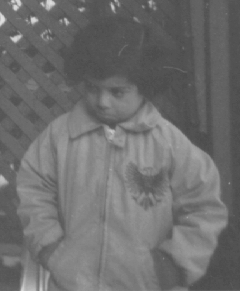
\includegraphics[width=\linewidth]{./result/baby.jpg}
        \caption{Original image}
      \end{subfigure}
      \hspace{1cm}
      \begin{subfigure}{.45\textwidth}
        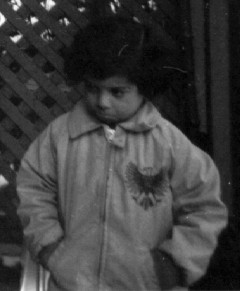
\includegraphics[width=\linewidth]{./result/labwork7-gpu-out.jpg}
        \caption{Greyscale stretched}
      \end{subfigure}
    \end{figure}
\end{itemize}
\section{Try experimenting with different 2D block size values}
\end{document}

